\PassOptionsToPackage{table}{xcolor}
\documentclass[xcolor=table]{beamer}
\usetheme{Madrid}
\usepackage{tikz, xcolor}
\usetikzlibrary{arrows.meta}
\usepackage{hyperref}
\usepackage{graphicx}
\title{Floyd's Algorithm: Shortest Path Problem}
\subtitle{Project 1}
\author{Daniel Romero - 2023059668 \break Adrián Zamora - 2023083307}
\institute[TEC]{\break Escuela de Ingeniería en Computación \break Instituto Tecnológico de Costa Rica \break Semester II 2025}
\date{September 12, 2025}
\begin{document}

\begin{frame}[plain]
\titlepage\end{frame}

\begin{frame}{Robert W. Floyd}
\begin{columns}
 \begin{column}{0.60\textwidth}
  \begin{itemize}
\item American computer scientist (1936 - 2001)
\item Studied physics at the University of Chicago, B.A. at age \textbf{19}
\item No formal CS degree → self-taught programming and algorithms
\item Worked as a math teacher, then in computing → professor at Stanford
\item Published foundational papers in computational theory
\item Collaborated with \textbf{Donald Knuth} on "The Art of Computer Programming"
\item Created cycle detection and \textbf{shortest paths} algorithms
\item Received the \textbf{Turing Award (1978)}
\end{itemize}
 \end{column}
 \begin{column}{0.40\textwidth}
\includegraphics[width=\linewidth,height=0.85\textheight,keepaspectratio]{Floyd/floyd-small.jpg}
 \end{column}
\end{columns}
\end{frame}

\begin{frame}{Floyd Algorithm (Floyd--Warshall Algorithm)}
  \begin{itemize}
    \item The Floyd Algorithm computes the \textbf{shortest paths between all pairs of nodes} in a graph with edge weights
    \item Works for both directed and undirected graphs
    \item \textbf{Time Complexity:} $O(n^3)$
      \begin{itemize}
        \item For each new node considered as an intermediate step, an entire $n \times n$ table is updated
      \end{itemize}
    \item \textbf{Space Complexity:} $O(n^2)$
      \begin{itemize}
        \item All calculations are performed within the same distance table
      \end{itemize}
    \item Based on the principle of \textbf{dynamic programming}
    \item It has applications in network routing and navigation systems
  \end{itemize}
  \begin{center}
    \includegraphics[width=0.35\textwidth,keepaspectratio]{Floyd/floydGraph.png}
  \end{center}
\end{frame}

\begin{frame}{Floyd Algorithm Overview}
  \begin{itemize}
    \item There are two tables: \textbf{D} and \textbf{P}.
    \item \textbf{D table:} stores distances between any two nodes.
      \begin{itemize}
        \item $D[i][i] = 0$ (distance from a node to itself).
        \item If edge $(i,j)$ exists, then $D[i][j] =$ weight of that edge, otherwise $D[i][j] = \infty$.
      \end{itemize}
    \item \textbf{P table:} stores path reconstruction information.
      \begin{itemize}
        \item P table is initialized with \textbf{0} on every cell (This means that there is a direct path between the two nodes)
      \end{itemize}
    \item \textbf{Algorithm process:}
      \begin{itemize}
        \item For each node $k = 1$ to $n$ (considered as an intermediate node):
        \item For each pair of nodes $(i,j)$, check if going through $k$ is shorter:
        \[
        D(k)[i][j] = \min\{D(k-1)[i][j],\; D(k-1)[i][k] + D(k-1)[k][j]\}
        \]
        \item Update $P[i][j]$ with the value k if there was a change in $D[i][j]$. (meaning we go through k to get from i to j)
      \end{itemize}
    \item After all iterations:
      \begin{itemize}
        \item $D$ contains shortest distances.
        \item $P$ contains the information to reconstruct the shortest paths.
      \end{itemize}
  \end{itemize}
\end{frame}

\begin{frame}{Graph}
\begin{center}
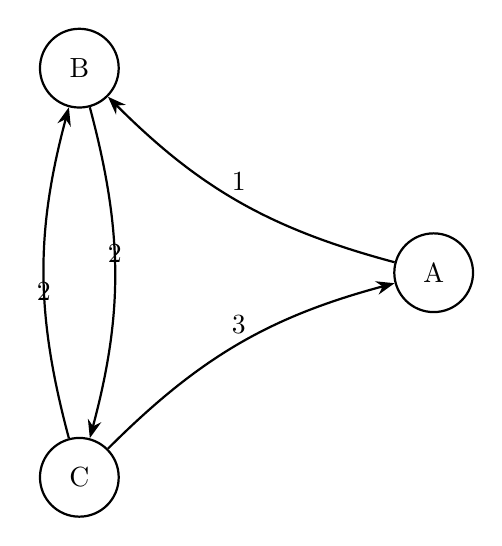
\begin{tikzpicture}[->, >=Stealth, thick, main/.style={circle, draw, minimum size=1cm}]

    \node[main] (A) at (0.00:3cm) {A};
    \node[main] (B) at (120.00:3cm) {B};
    \node[main] (C) at (240.00:3cm) {C};
\path
        (A) edge[bend left=15] node[above, fill=none] {1} (B)
        (B) edge[bend left=15] node[above, fill=none] {2} (C)
        (C) edge[bend left=15] node[above, fill=none] {3} (A)
        (C) edge[bend left=15] node[below, fill=none] {2} (B)
;
\end{tikzpicture}
\end{center}
\end{frame}

\begin{frame}{Table D(0)}
    \begin{center}
        \begin{tabular}{c|ccc}
         & A & B & C \\
\hline
A & 0 & 1 & $\infty$ \\
B & $\infty$ & 0 & 2 \\
C & 3 & 2 & 0 \\
        \end{tabular}
    \end{center}
\end{frame}

\begin{frame}{Table D(1)}
    \begin{center}
        \begin{tabular}{c|ccc}
         & A & B & C \\
\hline
A & 0 & 1 & $\infty$ \\
B & $\infty$ & 0 & 2 \\
C & 3 & 2 & 0 \\
        \end{tabular}
    \end{center}
\end{frame}

\begin{frame}{Table P}
    \begin{center}
        \begin{tabular}{c|ccc}
         & A & B & C \\
\hline
A & 0 & 0 & 0 \\
B & 0 & 0 & 0 \\
C & 0 & 0 & 0 \\
        \end{tabular}
    \end{center}
\end{frame}

\begin{frame}{Table D(2)}
    \begin{center}
        \begin{tabular}{c|ccc}
         & A & B & C \\
\hline
A & 0 & 1 & \textcolor{blue}{3} \\
B & $\infty$ & 0 & 2 \\
C & 3 & 2 & 0 \\
        \end{tabular}
    \end{center}
\end{frame}

\begin{frame}{Table P}
    \begin{center}
        \begin{tabular}{c|ccc}
         & A & B & C \\
\hline
A & 0 & 0 & \textcolor{blue}{2} \\
B & 0 & 0 & 0 \\
C & 0 & 0 & 0 \\
        \end{tabular}
    \end{center}
\end{frame}

\begin{frame}{Table D(3)}
    \begin{center}
        \begin{tabular}{c|ccc}
         & A & B & C \\
\hline
A & 0 & 1 & 3 \\
B & \textcolor{blue}{5} & 0 & 2 \\
C & 3 & 2 & 0 \\
        \end{tabular}
    \end{center}
\end{frame}

\begin{frame}{Table P}
    \begin{center}
        \begin{tabular}{c|ccc}
         & A & B & C \\
\hline
A & 0 & 0 & 2 \\
B & \textcolor{blue}{3} & 0 & 0 \\
C & 0 & 0 & 0 \\
        \end{tabular}
    \end{center}
\end{frame}

\begin{frame}{Shortest Paths from A}
\begin{itemize}
    \item to B (1): A $\rightarrow$ B
\item to C (3): A $\rightarrow$  B $\rightarrow$ C
\end{itemize}
\end{frame}

\begin{frame}{Shortest Paths from B}
\begin{itemize}
    \item to A (5): B $\rightarrow$  C $\rightarrow$ A
\item to C (2): B $\rightarrow$ C
\end{itemize}
\end{frame}

\begin{frame}{Shortest Paths from C}
\begin{itemize}
    \item to A (3): C $\rightarrow$ A
\item to B (2): C $\rightarrow$ B
\end{itemize}
\end{frame}

\end{document}